\documentclass[12pt]{article}
\usepackage[utf8]{inputenc}
\usepackage{mathtools, amsmath, amsthm, amssymb, graphicx, mathrsfs, verbatim}
%\usepackage[thmmarks, thref, amsthm]{ntheorem}
\usepackage{color}
\usepackage{wrapfig}
\usepackage{subcaption}
\usepackage[colorinlistoftodos,textsize=tiny]{todonotes} % need xargs for below
%\usepackage{accents}
\usepackage{bbm}
\usepackage{xspace}
\usepackage[margin=1.25in]{geometry}
\usetikzlibrary{calc}
\usepackage[colorlinks=true,breaklinks=true,bookmarks=true,urlcolor=blue,
     citecolor=blue,linkcolor=blue,bookmarksopen=false,draft=false]{hyperref}

\newcommand{\Comments}{1}
\newcommand{\mynote}[2]{\ifnum\Comments=1\textcolor{#1}{#2}\fi}
\newcommand{\mytodo}[2]{\ifnum\Comments=1%
  \todo[linecolor=#1!80!black,backgroundcolor=#1,bordercolor=#1!80!black]{#2}\fi}
\newcommand{\raf}[1]{\mynote{green}{[RF: #1]}}
\newcommand{\raft}[1]{\mytodo{green!20!white}{RF: #1}}
\newcommand{\jessie}[1]{\mynote{purple}{[JF: #1]}}
\newcommand{\jessiet}[1]{\mytodo{purple!20!white}{JF: #1}}
\newcommand{\btw}[1]{\mytodo{gray!20!white}{BTW: #1}}
\ifnum\Comments=1               % fix margins for todonotes
  \setlength{\marginparwidth}{1in}
\fi


\newcommand{\reals}{\mathbb{R}}
\newcommand{\posreals}{\reals_{>0}}%{\reals_{++}}

% alphabetical order, by convention
\newcommand{\D}{\mathcal{D}}
\newcommand{\E}{\mathbb{E}}
\newcommand{\F}{\mathcal{F}}
\newcommand{\I}{\mathcal{I}}
\renewcommand{\P}{\mathcal{P}}
\newcommand{\R}{\mathcal{R}}
\newcommand{\X}{\mathcal{X}}
\newcommand{\Y}{\mathcal{Y}}


\newcommand{\inter}[1]{\mathring{#1}}%\mathrm{int}(#1)}
\newcommand{\cl}[1]{\text{cl}(#1)}
%\newcommand{\expectedv}[3]{\overline{#1}(#2,#3)}
\newcommand{\expectedv}[3]{\E_{Y\sim{#3}} {#1}(#2,Y)}
\newcommand{\inprod}[2]{\langle #1, #2 \rangle}
\newcommand{\toto}{\rightrightarrows}
\newcommand{\trim}{\mathrm{trim}}
\newcommand{\fplc}{finite-piecewise-linear and convex\xspace} %xspace for use in text
\newcommand{\conv}{\mathrm{conv}}
\newcommand{\ones}{\mathbbm{1}}
\newcommand{\aff}{\text{aff}}
\newcommand{\im}{\text{im}}
\newcommand{\strip}{\mathrm{strip}}
\newcommand{\card}{\textbf{card}}
\newcommand{\simplex}{\Delta_\Y}

\DeclareMathOperator*{\argmax}{arg\,max}
\DeclareMathOperator*{\argmin}{arg\,min}
\DeclareMathOperator*{\arginf}{arg\,inf}
\DeclareMathOperator*{\sgn}{sgn}

\newtheorem{theorem}{Theorem}
\newtheorem{lemma}{Lemma}
\newtheorem{proposition}{Proposition}
\newtheorem{definition}{Definition}
\newtheorem{corollary}{Corollary}
\newtheorem{conjecture}{Conjecture}
\newtheorem{notation}{Notation}
\newtheorem{claim}{Claim}




\begin{document}
\section{Drawing relationship between polytopes and subgradients}
\subsection{Starting with a loss}
If we are given a loss $L$ and set of embedded reports (possible minimizers of the expected loss over $\P$), we know that $r \in \Gamma(p) \iff 0 \in \partial_r L(r, p)$.
We can represent $\partial_r L(r,p)$ as a (closed) polytope given by by $\{x \in \reals^d : Ax \leq b \}$ for some $A$ and $b$.

If $\Gamma$ is $d$-\emph{minimally}-embeddable, then for some $r$ and $p$, the polytope $\partial_r L(r,p)$ should be full-dimensional in $\reals^d$.

\subsection{Thinking on the property}
Each level set of a finite elicitable property can be described as a convex polytope, and we can give this cell as $\{p \in \simplex : B^ip \geq 0 \}$, so that the matrix $B^i$ describes cell $i$.
Observe the subtle restriction that $p \in \simplex$.
This imposes nonnegativity constraints and the restriction that $\sum_i y_i =1$.

To take care of nonnegativity constraints, we can build them into $B$.
That is, each row of $B$ should describe a supporting hyperplane of the cell.

To ensure that $\sum_i y_i = 1$, we can then also add two rows to $B$ and the vector of inequalities.
That is, we can add $\ones^T p \leq 1$ and $-\ones^T p \leq -1$.

So, if $B^* = \begin{Bmatrix}
B \\
\ones^T \\
-\ones^T
\end{Bmatrix}$ 
and $0^* = \begin{Bmatrix}
\vec{0}\\
1\\
-1
\end{Bmatrix}$
, then we can see that $\{p \in \simplex: Bp \geq \vec{0} \} = \{p \in \reals^n : B^* p \geq 0^*\}$.

However, the equality constraints just restrict to a subset of the original cell (not restricted to the simplex), so we know that $\{p \in \reals^n : B^* p \geq 0^*\} \subseteq \{p \in \reals^n : B p \geq 0\}$, and focus on the matrix $B$ instead of $B^*$.

\jessie{The difference between nonnegativity constraints and summing to $1$ is that we can construct an affine transformation to reduce dimension by $1$, guarantee the sum adds to $1$?}

Consider that the dual of a polyhedron $C$ is another polyhedron $T$ where the vertices of $T$ are each associated with a facet of $C$.
Since our cells $C^i$ are described by a set of linear inequalities, we know the (nonredundant) vectors describing these inequalities are associated with a facet of $C^i$, and are therefore also associated with a vertex of $T^i$.


i.e. For each facet of $C$, there should be a vector $v_j \in \reals^n$ so that the facet is described by the halfspace $\{x : \inprod{v_j}{x} \leq b_{i,j} \}$ for each column of $B^i$ 
Therefore, if the cell $C^i$ is described by $k$ halfspaces, then there should be at least $k$ vectors $v_j$

\jessie{Do we know anything about a lower bound on the number of normals needed?  Combining with structure of the properties might help us prove bounds.}

\section{Sidebar}
Not sure if this proof is obvious, but I haven't convinced myself the following statement is true yet, although I think it should be (or at least some variation of it):
\begin{claim}
For a finite elicitable property $\Gamma: \simplex\to\R$, the level set $\Gamma_r$ is a convex polytope in $\simplex$.
\end{claim}

\section{Characterizing possible loss functions}
If we can find a set of normals $V$ and $B^i$ matrices describing each cell $C^i$ of the property $\Gamma$ such that $T(\cdot, y) := \{x : \inprod{V}{x} \geq B_{i} \}$ is nonempty for each column $i$ of $B$, then the polytopes form subgradient sets of a possible loss function eliciting $\Gamma$.
\jessie{Still unknown: does $V$ have to be the same across cells?}

However, the loss function eliciting $\Gamma$ is almost never unique; in fact, it is not the only loss \emph{embedding} $\Gamma$, either.
The loss over reports in the convex hull of the embedded reports may be unique, but outside the convex hull, can take on infinitely many values, so long as it does not ``go below'' the minimum value of the embedded report.
One question to ask here is, given a set of normals $V \in \reals^{k \times d}$, is there a set of matrices $\{B^i\}_{i=1}^{n}$ so that $T(r,y)$ is nonempty for all $r$and $y$?

\jessie{Another way to frame this is to fix the matrices $B$ and find such a set of normals $V$, but my hunch says that the first way might be easier for constructions, and this might be easier for bounds?}


\section{Case study: abstain}
\subsection{Constructing $B$ and $V$}
Consider the cell $C$ describing a level set.
For finite elicitable properties, we know $C$ is a convex polytope \jessie{See Claim 1}, and can thus be understood as either the convex hull as a finite set of distributions in $\simplex$, or as the intersection of a finite set of half spaces.

First, we should note that the matrix $B$ can be written one of many ways.
The only requirement of $B$ is that it describes the cell with nonnegativity constraints.
It should be noted, however, that we can normalize $B$ so that the max element in each row is $1$.
That way, we can look at the polar of the set $V$, and the set of subgradients should be a subset of $V^\circ$.

\jessie{Options: Start with $V$ and reverse-engineer $B$ or start with any $B$ describing the cell and find a $V$ that describes it?}

For abstain(1/2) on 4 outcomes, consider the set of normals $V = \{(1,1), (-1,1), (-1,-1), (1,-1)\}$, \jessie{representing each of the embedded points?}.
The polar $V^\circ$ is then a diamond inscribed in the convex hull of the normals.
\begin{figure}
\begin{center}
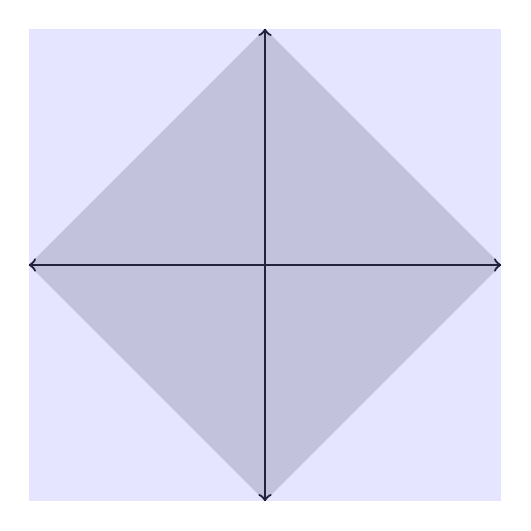
\begin{tikzpicture}[scale=3.0]
\draw[thick,->] (0,0) -- (0,-1);
\draw[thick,->] (0,0) -- (0,1);
\draw[thick,->] (0,0) -- (-1,0);
\draw[thick,->] (0,0) -- (1,0);

 \path[fill=gray, opacity=0.3] (0, 1) coordinate(p1) --  (-1, 0) coordinate(p2)
 -- (0, -1) coordinate(p3) --
 (1,0) coordinate(p4);
 
  \path[fill=blue, opacity=0.1] (1, 1) coordinate(c1) --  (-1, 1) coordinate(c2)
  -- (-1, -1) coordinate(c3) --
  (1,-1) coordinate(c4);
\end{tikzpicture}
\caption{$V^\circ$ in grey, $\conv(V)$ in blue.}
\label{fig:abstain-polar}
\end{center}
\end{figure}

For the abstain cell, we know that the matrix $B = \ones - 2I$ is unique up to scaling across rows. \jessie{I think... we haven't discussed or proved this.}
The polytopes $T(abs, \cdot)$ are then given as in Figure~\ref{fig:abstain-T-report-abs}.
\begin{figure}
\begin{minipage}{0.24\linewidth}
\begin{tikzpicture}[scale=1.5]
\draw[->] (0,0) -- (0,-1);
\draw[->] (0,0) -- (0,1);
\draw[->] (0,0) -- (-1,0);
\draw[->] (0,0) -- (1,0);
\draw[thick] (0, 1) --  (1, 0) ;
\end{tikzpicture}
\end{minipage}
\begin{minipage}{0.24\linewidth}
\begin{tikzpicture}[scale=1.5]
\draw[->] (0,0) -- (0,-1);
\draw[->] (0,0) -- (0,1);
\draw[->] (0,0) -- (-1,0);
\draw[->] (0,0) -- (1,0);
\draw[thick] (0, 1) --  (-1, 0) ;
\end{tikzpicture}
\end{minipage}
\begin{minipage}{0.24\linewidth}
\begin{tikzpicture}[scale=1.5]
\draw[->] (0,0) -- (0,-1);
\draw[->] (0,0) -- (0,1);
\draw[->] (0,0) -- (-1,0);
\draw[->] (0,0) -- (1,0);
\draw[thick] (0, -1) --  (1, 0) ;
\end{tikzpicture}
\end{minipage}
\begin{minipage}{0.24\linewidth}
\begin{tikzpicture}[scale=1.5]
\draw[->] (0,0) -- (0,-1);
\draw[->] (0,0) -- (0,1);
\draw[->] (0,0) -- (-1,0);
\draw[->] (0,0) -- (1,0);
\draw[thick] (0, -1) --  (-1, 0) ;
\end{tikzpicture}
\end{minipage}
\caption{$T(abs, \cdot)$ for each $y \in \Y$.}
\label{fig:abstain-T-report-abs}
\end{figure}

However, this embedding gets a little trickier when thinking about the other cells.
For each report of an outcome $r$, we know the matrix $B^r$ is not unique.
For example, for $r_1$, we can see either

\[ B_1 = \begin{bmatrix}
1 & -1 & -1 & -1 \\
0 & 1 & 0 & 0 \\
0 & 0 & 1 & 0 \\
0 & 0 & 0 & 1 \\
\end{bmatrix} 
% 
\text{ or }
B_2 = 
\begin{bmatrix}
1 & -1 & -1 & -1 \\
1 & 0 & 1 & 1 \\
0 & 1 & 1 & 1 \\
1 & 1 & 0 & 1 \\
\end{bmatrix} 
\]

describe the cell properly (with nonnegativity constraints).
However, these two constructions of the $B$ yield different polytopes $T(r_1, \cdot)$ for nearly all of the outcomes. (See Figures~\ref{fig:abstain-T-report-r1-B1} and \ref{fig:abstain-T-report-r1-B2}.)
This begs the question of what a \emph{minimal} and \emph{maximal} set of such polytopes would look like.
(For abstain(1/2) with $n=4$, I have a proof sketch that shows that the $B_1$ matrix gives the minimal set of polytopes where $0 \in T(r_1, p) \iff p \in \Gamma_{r_1}$.
I can sketch that out at another time.)


\begin{figure}
\begin{minipage}{0.24\linewidth}
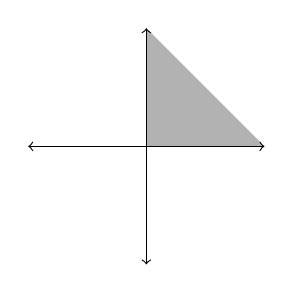
\begin{tikzpicture}[scale=1.5]
\draw[->] (0,0) -- (0,-1);
\draw[->] (0,0) -- (0,1);
\draw[->] (0,0) -- (-1,0);
\draw[->] (0,0) -- (1,0);
\path[fill=black, opacity=0.3] (0, 1) --  (0,0) -- (1,0) ;
\end{tikzpicture}
\end{minipage}
\begin{minipage}{0.24\linewidth}
\begin{tikzpicture}[scale=1.5]
\draw[->] (0,0) -- (0,-1);
\draw[->] (0,0) -- (0,1);
\draw[->] (0,0) -- (-1,0);
\draw[->] (0,0) -- (1,0);
\fill (-1,0) circle[radius=2pt];
\end{tikzpicture}
\end{minipage}
\begin{minipage}{0.24\linewidth}
\begin{tikzpicture}[scale=1.5]
\draw[->] (0,0) -- (0,-1);
\draw[->] (0,0) -- (0,1);
\draw[->] (0,0) -- (-1,0);
\draw[->] (0,0) -- (1,0);
\draw[thick] (0, -1) --  (-1, 0) ;
\end{tikzpicture}
\end{minipage}
\begin{minipage}{0.24\linewidth}
\begin{tikzpicture}[scale=1.5]
\draw[->] (0,0) -- (0,-1);
\draw[->] (0,0) -- (0,1);
\draw[->] (0,0) -- (-1,0);
\draw[->] (0,0) -- (1,0);
\fill (0,-1) circle[radius=2pt];
\end{tikzpicture}
\end{minipage}
\caption{$T(r_1, \cdot)$ for each $y \in \Y$ using the $B_1$ matrix.}
\label{fig:abstain-T-report-r1-B1}
\end{figure}


\begin{figure}
\begin{minipage}{0.24\linewidth}
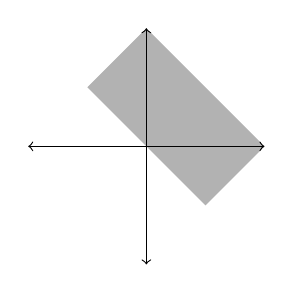
\begin{tikzpicture}[scale=1.5]
\draw[->] (0,0) -- (0,-1);
\draw[->] (0,0) -- (0,1);
\draw[->] (0,0) -- (-1,0);
\draw[->] (0,0) -- (1,0);
\path[fill=black, opacity=0.3] (0, 1) --  (-1/2,1/2) -- (1/2, -1/2) -- (1,0) ;
\end{tikzpicture}
\end{minipage}
\begin{minipage}{0.24\linewidth}
\begin{tikzpicture}[scale=1.5]
\draw[->] (0,0) -- (0,-1);
\draw[->] (0,0) -- (0,1);
\draw[->] (0,0) -- (-1,0);
\draw[->] (0,0) -- (1,0);
\draw[thick] (-1/2, -1/2) --  (-1, 0) ;
\end{tikzpicture}
\end{minipage}
\begin{minipage}{0.24\linewidth}
\begin{tikzpicture}[scale=1.5]
\draw[->] (0,0) -- (0,-1);
\draw[->] (0,0) -- (0,1);
\draw[->] (0,0) -- (-1,0);
\draw[->] (0,0) -- (1,0);
\draw[thick] (0, -1) --  (-1, 0) ;
\end{tikzpicture}
\end{minipage}
\begin{minipage}{0.24\linewidth}
\begin{tikzpicture}[scale=1.5]
\draw[->] (0,0) -- (0,-1);
\draw[->] (0,0) -- (0,1);
\draw[->] (0,0) -- (-1,0);
\draw[->] (0,0) -- (1,0);
\draw[thick] (0, -1) --  (-1/2, -1/2) ;
\end{tikzpicture}
\end{minipage}
\caption{$T(r_1, \cdot)$ for each $y \in \Y$ using the $B_2$ matrix.}
\label{fig:abstain-T-report-r1-B2}
\end{figure}


\section{Misc. thoughts}
\begin{itemize}
	\item I did some work to try to characterize the ``minimal'' polytopes by considering the set of distributions $\P$ such that the cell $C = \conv(\P)$.
	However, I would call it far from a proof.
	Thoughts on whether this is worth pursuing farther would be appreciated?
	
	\item For abstain, we might want an extra, redundant normal $(0,0) \in V$ so that the vectors of $V$ are the embedded reports?  
	(Requires getting rid of assumption that normals are in general position.)
	
	\item If $T$ is related to $C$ by some strong enough notion of duality, can we use the affine dimension of $C$ to draw conclusions about the affine dimension of $T$ (and therefore embedding dimension of $\Gamma$?) 
	
	\item Would it be plausible/desirable to write this as a convex program to find $V$ and $B$?

	\item It's sometimes hard to gain intuition because abstain has so much structure, I can't tell why some things are working out the way they are. (ex: normals corresponding to the embedded reports)
	
	\item Do we want to test this construction for ranking on 3 outcomes?
	
\end{itemize}



\end{document}
%%% Local Variables:
%%% mode: latex
%%% TeX-master: t
%%% End:


% % % % % % % % % % % % % % % % % % % % % % % % % % % % % % % % % %
% % % % % % % % % % % % % % % % % % % % % % % % % % % % % % % % % %
% % % % % % % % % % % % % % % % % % % % % % % % % % % % % % % % % %
% % % % % % % % % % % % % % % % % % % % % % % % % % % % % % % % % %
% % % % % % % % % % % % % % % % % % % % % % % % % % % % % % % % % %
% % % % % % % % % % % % % % % % % % % % % % % % % % % % % % % % % %
% % % % % % % % % % % % % % % % % % % % % % % % % % % % % % % % % %
% % % % % % % % % % % % % % % % % % % % % % % % % % % % % % % % % %
% % % % % % % % % % % % % % % % % % % % % % % % % % % % % % % % % %
% % % % % % % % % % % % % % % % % % % % % % % % % % % % % % % % % %
% % % % % % % % % % % % % % % % % % % % % % % % % % % % % % % % % %
% % % % % % % % % % % % % % % % % % % % % % % % % % % % % % % % % %
% % % % % % % % % % % % % % % % % % % % % % % % % % % % % % % % % %
% % % % % % % % % % % % % % % % % % % % % % % % % % % % % % % % % %
% % % % % % % % % % % % % % % % % % % % % % % % % % % % % % % % % %


\section{Fun Trim proofs}
\subsection{Notation and Definitions}


A set of level sets $\Theta$ is an unlabeled property, and finite if $|\Theta| < \infty$.

\jessiet{COmmented out definition of strip}
%\begin{definition}
%Let $\Gamma:\P\toto\R$.
%Define $\text{strip}(\Gamma) := \{ \Gamma_r : r \in \R \}$.
%\end{definition}
%Informally, strip removes labels from the property.
%\btw{Strip includes the boundaries of level sets / lower dimensional level sets.}

\begin{notation}
Let $\gamma: \P \toto\R$ and $\Gamma: \P \toto\reals^d$.
We say $\gamma \preceq \Gamma$ if for all $p \in \P$, we observe $\gamma(p) = \Gamma(p) \cap \R$.
\end{notation}

\begin{definition}
	The elicitable property $\Gamma:\P\toto \reals^d$ is a \emph{d-embedding} of $\gamma: \P \toto \R$ if there exists an injection $\varphi:\R \to \reals^d$ such that $\varphi(r) \in \Gamma(p) \iff r \in \gamma(p)$. 
\end{definition}

%Note that we can take $\varphi^{-1}(r') = \{ r \in \R: \varphi(r) = r' \}$.
%That is, we define the inverse of $\varphi$ as a possibly set-valued function.

\begin{definition}
	A level set $\theta$ is \emph{full-dimensional} if it has nonempty interior.
\end{definition}


\subsection{Lemmas on the way}

\begin{lemma}\label{lem:gam-prime-exists}
	Let $\Gamma:\P \toto \reals^d$ be a nondegenerate elicitable property with a finite set of full-dimensional level sets $\Theta$ so that $\bigcup_{\theta \in \Theta}\theta = \P$.
	There exists a nondegenerate, nonredundant property $\gamma: \P \toto \R$ such that $\gamma \preceq \Gamma$. 
\end{lemma}
\begin{proof}
	Construct the finite set $\R = \{[u] \in \Gamma(p) : p \in \inter{\theta} \}_{\theta \in \Theta}$, where $[u]$ is one consistent report for all the reports $r, r'$ such that $\Gamma_r = \Gamma_{r'}$. 
	Defining the property $\gamma : p \mapsto \Gamma(p) \cap \R$, we see that $\gamma \preceq \Gamma$.
	We want to show that the constructed $\gamma$ is nondegenerate and nonredundant.

	As $\Gamma$ is nondegenerate, there is some report $u \in \reals^d$ such that $u \in \Gamma(p)$ for all $p\in\P$, so $[u] \in \gamma(p)$ and is well-defined for all $p \in \P$.
	Thus, $\gamma$ is nondegenerate.

	To see $\gamma$ is nonredundant, first consider two reports $u_1, u_2$ such that $\Gamma_{u_1} = \Gamma_{u_2}$.
	In this case, $[u_1] = [u_2] = r$, so $\gamma_{r} = \gamma_{r}$ does not lead to a redundant report.
	
	\jessiet{This is the part I'm least confident about... see Lemma~\ref{lem:nonempty-inter-iff-aff-ind}}
	Now, suppose there were reports $r, r' \in \R$ so that $\gamma_{r} \subsetneq \gamma_{r'}$.
	By construction of $\R$, both $\gamma_{r'}$ and $\gamma_r$ are full dimensional.
	For each elicitable property, there is a convex scoring rule $G:\Delta_\Y \to \reals$ with a bijection between the subgradients of $G$ and reports in $\R$ (one we reduce to equivalent reports-- see Theorem~\ref{thm:bij-loss-to-score}).
	As $G$ is convex, it must be differentiable almost everywhere. 
	However, for every distribution $p \in \gamma_{r'} = \gamma_{r} \cap \gamma_{r'}$, the subgradient of $\partial G(p)$ is set-valued, and therefore $G$ is not differentiable, on this set of positive Lebesgue measure in the simplex. 
	Contradicting the elicitability of $\gamma$, we conclude $\gamma$ is nonredundant. 

	Therefore, our constructed $\gamma$ is nondegenerate, nonredundant, and $\gamma \preceq \Gamma$.
\end{proof}

\jessiet{Revisit this with the paper's definition of trim}
\begin{lemma}\label{lem:define-trim}
	Let $\Gamma:\P\toto\reals^d$  be a nondegenerate, elicitable property with a finite set of level sets $\Theta$ so that $\bigcup_{\theta \in \Theta} \theta = \P$.
	There exists an unlabeled property $\Theta$ so that for all nondegenerate, nonredundant $\gamma \preceq \Gamma$, we have $\strip(\gamma) = \Theta := \trim(\Gamma)$.
\end{lemma}

\begin{proof}
	Let $\gamma:\P \toto \R$ and $\Gamma' : \P \toto \R'$ be nondegenerate, nonredundant properties so that $\gamma \preceq \Gamma$ and $\Gamma'\preceq \Gamma$.
	We want to show $\strip(\gamma) = \strip(\Gamma')$ in order to conclude that $\trim(\Gamma)$ is unique.
	For each $r \in \R$, there is a set of reports in $S \subseteq \reals^d$ so that there is a full-dimensional level set $\theta = \bigcap_{u\in S}\Gamma_s$ and $r = [u]$ for every $u \in S$.
	For the same set of reports $S$, we can equivalently choose a (possibly different) representative report $r' \in \R'$ so that $r' = [u]$ for every $u \in S$, since $\Gamma' \preceq \Gamma$.
	
	There is a bijection $\varphi : \R \to \R'$ so that $\varphi(\gamma(p)) = \Gamma'(p)$ for all $p \in \P$.
	Thus, the level sets of each report are the same since they are restrictions of the same property, as $\strip(\gamma) = \{ \gamma_r : r \in \R \} = \{ \Gamma_r : r \in \R \} = \{ \Gamma_{\varphi(r)} : r \in \R \} = \{ \Gamma_r : r \in \R' \} = \strip(\Gamma')$.
\end{proof}

\begin{lemma}\label{lem:lev-sets-subsets}
	Let the property $\Gamma: \P \toto \reals^d$ be elicitable and the nondegenerate, nonredundant property $\gamma: \P \toto \R$ so that $\gamma \preceq \Gamma$.
	Then the level sets of $\Gamma$ are subsets of the level sets of $\gamma$.
\end{lemma}

\begin{proof}
	It is sufficient to show $\theta \in \strip(\Gamma) \implies \theta \in \strip(\gamma)$.
	Given $\theta \in \strip(\Gamma)$, there is some report $u \in \reals^d$ so that $u \in \Gamma(p)$ for every $p \in \theta$.
	For every $r \in \R$, recall that there is an $u \in \reals^d$ so that $r = [u]$.
	By definition, $u \in \Gamma(p) \implies [u] = r \in \gamma(p)$.
	Therefore, there is some $r \in \R$ so that $p \in \Gamma_u \implies p \in \Gamma_{[u]} = \gamma_{r}$.
\end{proof}

\begin{proposition}\label{prop:optimal-reports-per-level-set}
  Let $\Gamma:\P\toto\reals^d$ be a non-degenerate (convex) elicitable property.

  The following are equivalent:
  \begin{enumerate}
  \item There is a nondegenerate, finite property $\gamma:\P\toto\R$ such that there is an injection $\varphi:\R\to\reals^d$ such that $r\in\gamma(p) \iff \varphi(r) \in \Gamma(p)$. (i.e. $\Gamma$ embeds finite $\gamma$).  
  \item $\trim(\Gamma)$ is finite.     
  \item There is a finite set of full-dimensional level sets $\Theta$ of $\Gamma$ that union to $\P$.

  \end{enumerate}
\end{proposition}

\begin{proof}
We proceed in a cycle to show $1 \implies 2 \implies 3 \implies 1 $.
\begin{enumerate}


\item [$1 \implies 2$]

We know $\strip(\gamma) = \trim(\Gamma)$ (since $\varphi$ is an injection, and there is some intermediate property $\Gamma'$ such that $\Gamma' \preceq \Gamma$ and with a bijection $\phi:\Gamma'(p) \mapsto \gamma(p)$, so $\strip(\Gamma') = \strip(\gamma)$.) 
As $\gamma$ is finite, so is $\strip(\gamma)$ since strip is generated from the (finite) report set.

\item [$2 \implies 3$]
Since $\Gamma$ is nondegenerate and every $\theta \in \trim(\Gamma)$ is full dimensional, it is clear that the union of the (full-dimensional) level sets of $\trim(\Gamma)$ union to $\P$ by nondegneracy of $\Gamma$.
	

\item[$3 \implies 1$]
Construct $\R := \{[u] \in \Gamma(p) : p \in \inter{\theta} \}_{\theta \in \Theta}$.
The property $\gamma: p \mapsto \Gamma(p) \cap\R$ is then finite as $\R$ is finite.
Taking $\varphi$ to be the identity, $\Gamma$ embeds this finite $\gamma$.
\end{enumerate} 

\end{proof}


\section{Lemmas probably not necessary for the paper}

\begin{lemma}\label{lem:nonempty-inter-iff-aff-ind}
	Let $\theta$ be a [closed] convex level set.
	The following are equivalent:
	\begin{enumerate}
		\item $\theta$ is full-dimensional
		\item $m(\theta) > 0$
		\item There are distributions $p_1, p_2, \ldots, p_n \in \theta$ so that $p_1, p_2, \ldots, p_n$ are affinely independent.
	\end{enumerate}
\end{lemma}
\begin{proof}
	Recall that $n := |\Delta_{\Y}|$, so we say the simplex is $n$-dimensional.
	\begin{enumerate}
		\item [$1 \implies 2$]
		A convex set that is full-dimensional contains the $\epsilon$-ball, since it has nonempty interior, and this ball has positive measure.
		
		\item [$2 \implies 3$]
		A convex set of positive measure contains the $\epsilon$-ball, which is the superset of the convex hull of a $n$ affinely independent points, and thus contains those points.
		
		\item [$3 \implies 1$]
		Let the set of distributions $Q := \{q_i\}_{i=1}^n$ be affinely independent, where each $q_i \in \theta$.
		Since the set $\theta$ is convex, then $\conv(Q) \subseteq \theta$.
		Let $q_1, q_2 \in Q$ so that $q_1 \neq q_2$.
		As $p = \sum_{i=1}^n \frac{1}{n}q_i \in \conv(Q)$, as is every $q \in B(\epsilon, p)$ since they are also convex combinations of elements of $Q$, we can see $\emptyset \neq \inter{\conv(Q)} \subseteq \inter{\theta}$, so we conclude $\theta$ is full-dimensional.
	\end{enumerate}
\end{proof}

\begin{theorem}[F/K 2014] \label{thm:bij-loss-to-score}
	Let $\Gamma: \P \toto\R$ be nonredundant and elicited by $\Gamma$-regular \jessiet{Can we assume this with convex elicitability? I read $\Gamma$-regular to mean that $L(r,p) < \infty$ for all $r \in \R$.} affine loss $L: \R \times \P \to \reals$ be given.
	Then $L$ elicits $\Gamma$ if and only if there exists some convex $G: \conv(\P) \to \reals$ with $G(\P) \subseteq \reals$, some $\D \subseteq \partial G$, and a bijection $\varphi : \R \to \D$ so that $\Gamma(t) = \varphi^{-1}(\D \cap \partial G_t)$.
\end{theorem}

